\documentclass[10pt,a4paper,twocolumn,twoside]{article}
\usepackage[utf8]{inputenc}
\usepackage[catalan]{babel}
\usepackage{multicol}
\usepackage{graphicx}
\usepackage{fancyhdr}
\usepackage{times}
\usepackage{titlesec}
\usepackage{url}
\usepackage{multirow}
\usepackage{lettrine}
\usepackage[top=2cm, bottom=1.5cm, left=2cm, right=2cm]{geometry}
\usepackage[figurename=Fig.,tablename=TAULA]{caption}
\captionsetup[table]{textfont=sc}

\author{\LARGE\sffamily Miquel Freixes Faya}
\title{\Huge{\sffamily Anàlisis de la relació entre les emisions de Co2 i l'augment de la temperatura, mitjançant tècniques i tecnologies de Big Data. 1r Informe de Seguiment}}
\date{}

\newcommand\blfootnote[1]{%
  \begingroup
  \renewcommand\thefootnote{}\footnote{#1}%
  \addtocounter{footnote}{-1}%
  \endgroup
}

%
%\large\bfseries\sffamily
\titleformat{\section}
{\large\sffamily\scshape\bfseries}
{\textbf{\thesection}}{1em}{}

\begin{document}

\fancyhead[LO]{\scriptsize MIQUEL FREIXES FAYA: TÍTOL DEL TREBALL}
\fancyhead[RO]{\thepage}
\fancyhead[LE]{\thepage}
\fancyhead[RE]{\scriptsize EE/UAB TFG INFORMÀTICA: TÍTOL (ABREUJAT SI ÉS MOLT LLARG)}

\fancyfoot[CO,CE]{}

\fancypagestyle{primerapagina}
{
   \fancyhf{}
   \fancyhead[L]{\scriptsize TFG EN ENGINYERIA INFORMÀTICA, ESCOLA D'ENGINYERIA (EE), UNIVERSITAT AUTÒNOMA DE BARCELONA (UAB)}
   \fancyfoot[C]{\scriptsize ``Febrer'' de 2019, Escola d'Enginyeria (UAB)}
}

%\lhead{\thepage}
%\chead{}
%\rhead{\tiny EE/UAB TFG INFORMÀTICA: TÍTOL (ABREUJAT SI ÉS MOLT LLARG)}
%\lhead{ EE/UAB \thepage}
%\lfoot{}
%\cfoot{\tiny{February 2015, Escola d'Enginyeria (UAB)}}
%\rfoot{}
\renewcommand{\headrulewidth}{0pt}
\renewcommand{\footrulewidth}{0pt}
\pagestyle{fancy}

%\thispagestyle{myheadings}
\twocolumn[\begin{@twocolumnfalse}

%\vspace*{-1cm}{\scriptsize TFG EN ENGINYERIA INFORMÀTICA, ESCOLA D'ENGINYERIA (EE), UNIVERSITAT AUTÒNOMA DE BARCELONA (UAB)}

\maketitle

\thispagestyle{primerapagina}
%\twocolumn[\begin{@twocolumnfalse}
%\maketitle
%\begin{abstract}
\begin{center}

{\vrule depth 0pt height 0.5pt width 4cm\hspace{7.5pt}%
\raisebox{-3.5pt}{\fontfamily{pzd}\fontencoding{U}\fontseries{m}\fontshape{n}\fontsize{11}{12}\selectfont\char70}%
\hspace{7.5pt}\vrule depth 0pt height 0.5pt width 4cm\relax}

\end{center}

\bigskip
%\end{abstract}
\end{@twocolumnfalse}]

\blfootnote{$\bullet$ E-mail de contacte: m.freixes.faya@gmail.com}
\blfootnote{$\bullet$ Menció realitzada: Tecnologies de la Informació}
\blfootnote{$\bullet$ Treball tutoritzat per: Jordi Casas Roma (departament)}
\blfootnote{$\bullet$ Curs 2018/19}

\section{Evolució dels Objectius}
\lettrine[lines=3]{L}{'objectiu} principal d'aquest treball segueix sent el mateix que el esmentat anteriorment, analitzar el canvi de temperatura al llarg dels anys. El que si que ha canviat són parametres amb els que es compararà la temperatura. Enlloc de fer-ho amb la petjada ecològica i les emisions de Diòxid de Carboni (CO$_2$), com s'havia plantejat en un inici, es farà amb les emisions de tres gasos hivernacles. També s'ha decidit reduïr l'area d'on s'agafaran les dades, enlloc de fer-ho de tota la Terra es focalitzarà en el continent d'Europa, concretament en els països dins de la Unió Europea.

El primer canvi s'ha decidit després d'analitzar els \textit{DataSets} amb més detall i veure que tenia més sentit comparar els canvis de temperatura amb les principals causes que podien provocar-los. Per tant s'ha decidit agafar només les dades sobre les emisions de  CO$_2$, les de Metà (N$_2$O) i les de  La comparació inicial també complicava bastant el treball,degut a la complexitat de les fòrmules i conceptes involucrats en el \textit{DataSet} de  la petjada ecològica. Com el treball està enfocat en el tractament de les dades i al seu anàlisi, s'ha trobat més coherent agafar conceptes menys complicats per  poder dedicar més temps en el seu processament. 

El segon té una justificació semblant, agafant els països dins de la Unió Europea s'obtenen unes 22000 files d'informació i agafar més països hagués produït un augment del temps d'entrenament de l'algorisme Això causaria una extensió de la planificació. Com s'ha esmentat anteriorment, com l'objectiu es dins de l'àmbit informàtic, hi ha suficient amb un gruix de dades de més de 20000 files per asolir-lo, per tant es descartaran la resta de països. A més a Europa hi ha una combinació de països curiosa, ja que hi ha alguns que han reduït dràsticament les emisions mentres d'altres que les han anat pujant o mantingut al llarg dels anys. 

\section{ Evolució de la Planificació}
La planificació s'està seguint tal com es va acordar. Hi ha un retard daproximadament una setmana degut a que no es va considerar la redacció dels informes, a la figura 1 es mostra el Diagrama de Gantt actualitza't amb les tasques dels informes afegides. 

\section{Evolució de la Metodologia}

\section{Preprocessament de dades}

\begin{thebibliography}{11}
\bibitem{1}
\url{https://www.kaggle.com/unitednations/international-greenhouse-gas-emissions}
\bibitem{2}
\url{https://www.kaggle.com/footprintnetwork/national-footprint-accounts-2018}

\bibitem{3}
"Ecological Footprint", \textit{WWF}. [En línia]. Disponible a: \url{https://wwf.panda.org/knowledge_hub/teacher_resources/webfieldtrips/ecological_balance/eco_footprint/}. [Accedit Octubre 4, 2018].
 
\bibitem{4}
"Sample Research", \textit{The Standish Group}.~[En~línia].~Disponible~a:~\url{https://www.standishgroup.com/sample_research}~[Accedit~Octubre~4,~2018].

\bibitem{5}
"Scrum Reference Card now available in English and Spanish",  \textit{Agile Methodology}. [En línia]. Disponible a: \url{http://agilemethodology.org/ }. [Accedit Octubre 4, 2018].

\bibitem{6}
"The Complete Guide to Understanding Agile Testing", \textit{QA Symphony}. [En línia].Disponible a: \url{https://www.qasymphony.com/blog/agile-methodology-guide-agile-testing/}. [Accedit Octubre 4, 2018].

\bibitem{7}
A.Géron, \textit{Hands-On Machine Learning with Scikit-Learn \& TensorFlow}. Sebastopol, CA: O’Reilly Media, 2017.

\bibitem{8}
"Supervised Learning", \textit{Scikit-Learn}. Disponible a: \url{http://scikit-learn.org/stable/supervised_learning.html#supervised-learning}. [Accedit Octubre 5, 2018].
\end{thebibliography}
\clearpage
\section{Annex}

\begin{figure}[!h]
\centering
	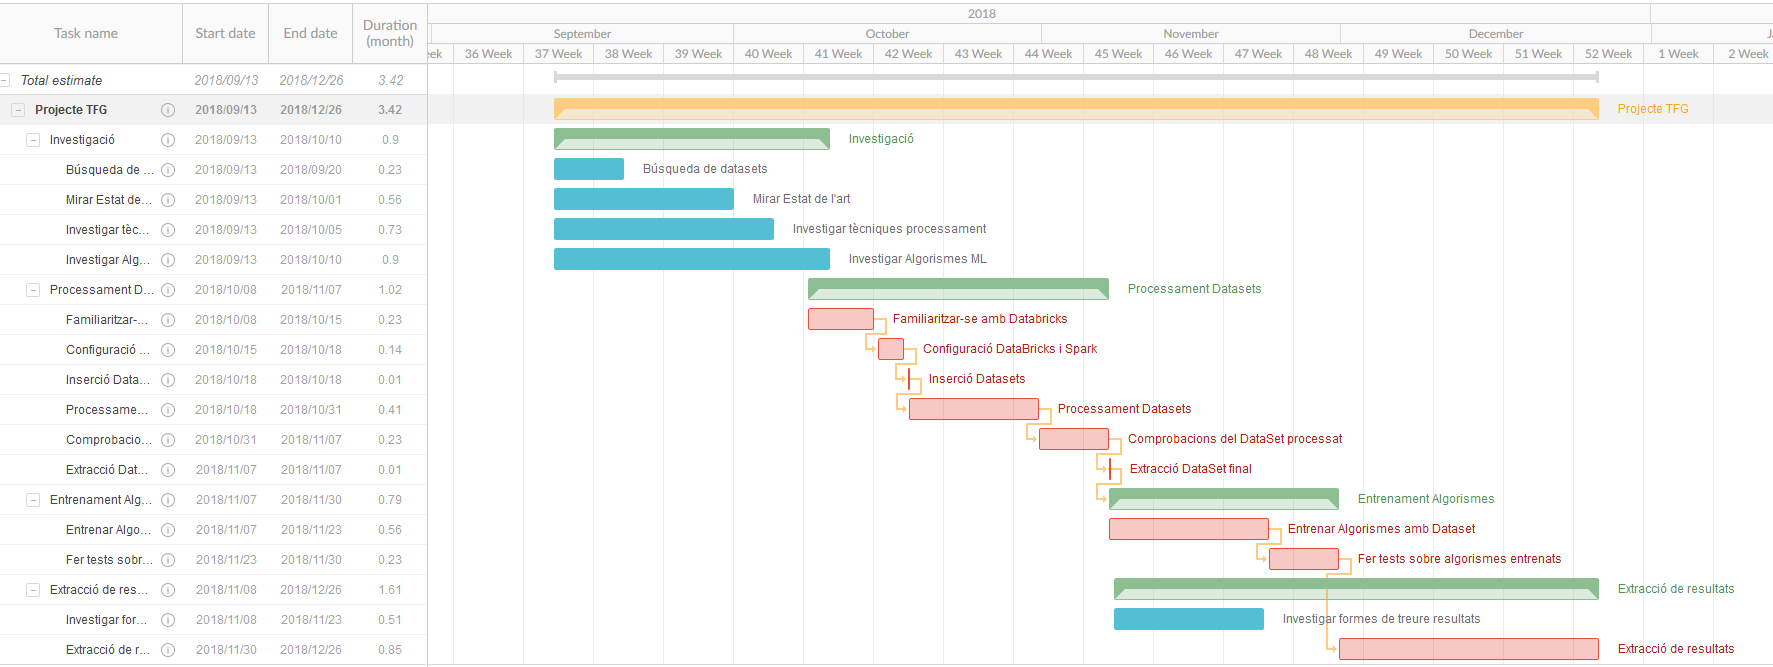
\includegraphics[width=1\textwidth]{img/diagrama_Gantt}

	\caption{Diagrama de Gantt}
	\label{fig-Gantt}
\end{figure}


\end{document}

